%-------------------------------------------------------------------------------
\chapter{Balance of a humanoid robot}
\label{ch.balance}
\acresetall
%-------------------------------------------------------------------------------

One of the primary topics of the present thesis is preservation of balance by
humanoid robots. Though this problem has been studied extensively, the definition of
balance itself is often too vague or is limited to a particular application,
such as walking. Therefore, we start by defining the balance preservation
problem in a general and informal way using the concepts of \tn{viability
theory} \cite{Aubin2011viability}, which has already been employed in
\cite{Wieber2002stability, Koolen2012ijrr, Zaytsev2015icra}. Thereafter we
discuss other related concepts in robotics and control and interpret the
existing approaches to balance preservation using the viability concepts.



%%%%%%%%%%%%%%%%%%%%%%%%%%%%%%%%%%%%%%%%%%%%%%%%%%%%%%%%%%%%%%%%%%%%%%%%%%%%%%%%
%%%%%%%%%%%%%%%%%%%%%%%%%%%%%%%%%%%%%%%%%%%%%%%%%%%%%%%%%%%%%%%%%%%%%%%%%%%%%%%%
%%%%%%%%%%%%%%%%%%%%%%%%%%%%%%%%%%%%%%%%%%%%%%%%%%%%%%%%%%%%%%%%%%%%%%%%%%%%%%%%
\section{Balance preservation as a viability problem}\label{sec.balance_as_viability}

Consider a general dynamical system
%
\begin{subequations}\label{eq.general_system}
\begin{empheq}[left=\empheqlbrace]{align}
    \dotV{x} &= f(\V{x}, \V{u}, t), \\
    \V{x} &\in \SET{X}(\V{x},t) \subset \RR^{n}, \\
    \V{u} &\in \SET{U}(\V{x},t) \subset \RR^{m},
\end{empheq}
\end{subequations}
%
where $\V{x}$ and $\V{u}$ are the state and control vectors subject to varying
constraints. Violation of the constraints indicates a failure, \IE, an
undesirable or infeasible state-control pair. An infinitely long evolution of
the $(\V{x}, \V{u})$ pair is called \tn{viable}, if it always complies with the
constraints, and, hence, never results in a failure. Accordingly, we call a
state $\V{x}$ \tn{viable}, if at least one viable evolution starts from it. All
viable states define the \tn{viability kernel} $\SET{V}$. In practice, we are
interested in reaching some \tn{target set} $\SET{T} \subset \SET{V}$. The set
of states from which the target can be reached is referred to as the
\tn{capture basin} $\SET{C}$ ($\SET{T} \subset \SET{C} \subset \SET{V}$). For
convenience, we also introduce the set $\SET{C}_H \subset \SET{C}$, such that
the target can be reached from it within a time interval $H$. Whenever $\V{x}
\in \SET{C}$ we call $\V{x}$ \tn{capturable}.

%
\begin{figure}[ht]
    \centering{%
    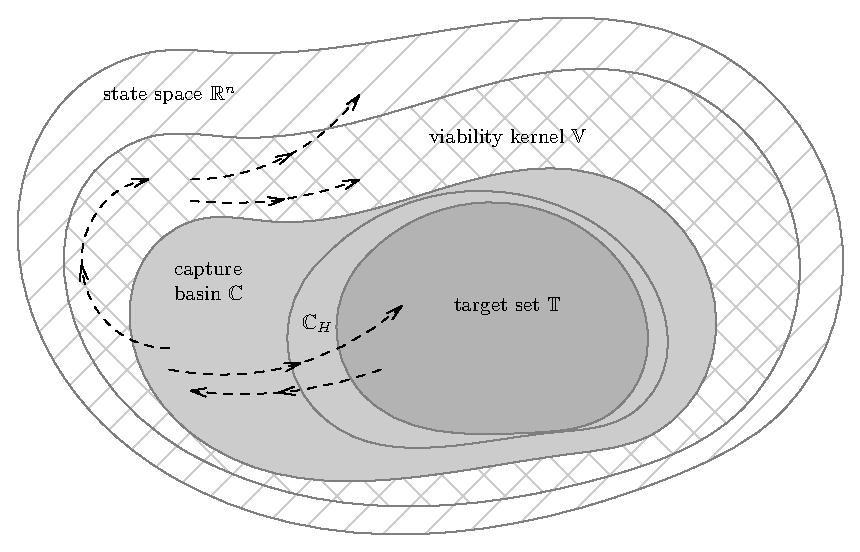
\includegraphics{viability.eps}}
    \caption[Viability kernel, capture basin, and target set.]{
        Viability kernel, capture basin, and target set. Possible evolutions
        are shown with dashed curves.
    }
    \label{fig.viability}
\end{figure}
%


Intuitively, preservation of balance means avoiding \tn{falls} at all future
moments. This definition immediately suggests interpretation using the
viability concepts presented above. Let us assume that we have a set of
constraints, violation of which indicates a fall. Then the balance is ensured
if the state of the robot stays within the viability kernel $\SET{V}$
constructed based on these constraints. In general, it is difficult to check if
a state is inside of the viability kernel, since the computation of $\SET{V}$
appears to be intractable in the case of such complex systems as humanoid
robots \cite{Wieber2002stability}. However, it is usually possible to isolate a
target subset $\SET{T} \subset \SET{V}$ consisting of states, which can be
easily demonstrated to be balanced. For example, $\SET{T}$ may contain states,
in which the robot is stopped, or states comprising a cycle in $\SET{V}$. Later
in this chapter we will see that all common approaches to balance preservation
explicitly or implicitly make use of $\SET{T}$ or the respective capture basin
$\SET{C}$.


Generally speaking, falling is not the only type of a failure, which may happen
to a robot. Depending on the context, failures may be defined as violations of
hardware limits, collisions with the environment, and even undesirable
behaviors, such as bending of the torso while walking. If these failures can
be indicated by some constraints, they can also be described in terms of
viability theory. Therefore, while controlling the robot we should aim at
staying within the viability kernel $\SET{V}$ defined with respect to
constraints reflecting all possible failures. However, in practice it is
usually necessary to consider constraints of different types separately in
sequential schemes for control or planning to tackle the concomitant
computational complexity. In the rest of the thesis the sets $\SET{V}$,
$\SET{C}$, and $\SET{T}$ always take into account the constraints due to
balance preservation and, optionally, other constraints, which are added
depending on the context. Thus, by saying that a particular state is viable or
capturable we imply that a fall can be avoided starting from it.


Though the main control goal is to avoid failures and, in particular, preserve
balance, we argue that this is not sufficient in practice, since we almost
always want the robot to eventually stop, or at least be able to stop. In other
words, the ultimate control goal is not to stay within $\SET{V}$, but rather to
stay within the capture basin $\SET{C}$ corresponding to the target set
$\SET{T}$ composed of the states in which the robot is stopped. This choice of
control goal may appear to be of a philosophical importance due to negligible
difference between the capture basin $\SET{C}$ and viability kernel $\SET{V}$
constructed for some simplified models of humanoid robots
\cite{Zaytsev2015thesis}. However, our point of view has an advantage when it
is necessary to design a controller without explicit knowledge of $\SET{C}$ and
$\SET{V}$: ensuring $\V{x} \in \SET{C}_H$ is easier than $\V{x} \in \SET{V}$.



%%%%%%%%%%%%%%%%%%%%%%%%%%%%%%%%%%%%%%%%%%%%%%%%%%%%%%%%%%%%%%%%%%%%%%%%%%%%%%%%
\subsection{Related terms and concepts}

Legged locomotion is one of the most common tasks of humanoid robots. At the
same time, stepping allows to compensate for perturbations, for example,
pushes. For these reasons, the general problem of balance preservation is often
perceived as a problem of making proper steps. The number of steps required to
stop the robot, and positions of these steps are of particular interest, which
was recognized as early as 70's \cite{Yamashita1974robman}. Consequently,
suitable terminology was introduced in the recent works
\cite{Pratt2006fastmotions, Koolen2012ijrr}, where a certain state is called
$K$-\tn{step capturable}, if the robot can stop by making no more than $K$
steps. Though this term does not originate from viability theory, it does not
contradict with the definition of capturability given above. In particular, the
relation between the capture basin $\SET{C}$ when the target is to stop the
robot and the set of $K$-step capturable states $\SET{K}_K$ is described by
%
\begin{equation}\label{eq.Kcapturability}
    \SET{C} = \bigcup_{K \ge 0} \SET{K}_K.
\end{equation}
%
Some researchers focused on the case, when it is necessary to maintain a
desired walking or running cycle \cite{Carver2009chaos, Zaytsev2015icra}.
Carver studied $K$-\tn{step deadbeat} control laws, which allow to compensate
for disturbances in $K$ steps while running \cite{Carver2009chaos}. Zaytsev
introduced $K$-\tn{step controllability} as generalization of $K$-step
capturability to the cases, when the goal can also be to maintain a given
walking speed \cite{Zaytsev2015thesis}. This case can also be described using
the notion of capturability as defined here: the relation between the set of
$K$-step controllable states and the capture basin is equivalent to
\cref{eq.Kcapturability}.


Viability theory can be applied to many problems in robotics. Hence, it is not
surprising, that some of the application-specific terminology introduced in the
field is equivalent to the notions of viability or capturability. For example,
\tn{inevitable collision states} defined in the context of collision avoidance
comprise the complement of a viability kernel \cite{Fraichard2003iros}. Another
example is the \tn{alternative safe behaviors} constructed in
\cite{Rubrecht2012auro} to avoid violation of the control constraints of a
manipulator. These behaviors are to be triggered to safely stop the robot, when
there is no other way to avoid violation of the constraints. Essentially, this
allows to maintain capturability at all times. Schouwenaars introduced
\tn{terminal feasible invariant sets}, ``\tn{in which a vehicle can remain for
an indefinite period of time without colliding with obstacles or other
vehicles}'', \IE, without violating constraints of the system
\cite[Chapter~4]{Schouwenaars2006thesis}. These sets are conceptually equivalent
to the target sets $\SET{T}$ considered here. Consequently, existence of a
trajectory, which ends in a terminal feasible invariant set, establishes that
the current state of a vehicle is capturable with respect to the system
constraints.


Related concepts are also used in general control theory. For example,
\tn{recursive feasibility} property of \ac{MPC} implies feasibility with
respect to constraints at each future control iteration
\cite[Chapter~8]{Rossiter2003mpc}. Hence, recursive feasibility implies
viability. Some researchers have already pointed out the connection between
viability theory and the notions of \tn{controllability} and \tn{reachability}
\cite{Zaytsev2015icra, Wieber2015handbook} or \tn{control invariant sets}
\cite{Wieber2002stability}. Typically, these notions are employed for simple
cases of linear systems or systems with non-varying constraints
\cite{Sontag1998control, Blanchini2008sets, Borrelli2015mpc,
Kerrigan2000thesis}. As a result, there exists a vast variety of extensions and
specifications meant to adapt controllability, reachability, or control
invariant sets to nonlinear and hybrid systems \cite{Sontag1998control,
Tomlin2003procieee, Bemporad2000tranac, Lewis1999siamr}, to obstacle avoidance
constraints \cite[Chapter~15]{LaValle2006planning} or general varying
constraints \cite[Chapter~2]{Rawlings2009mpc}. We believe that such variety may
lead to a confusion, which can only be resolved by rigorous definitions. For
this reason, here we resort to the concepts of viability theory.



%%%%%%%%%%%%%%%%%%%%%%%%%%%%%%%%%%%%%%%%%%%%%%%%%%%%%%%%%%%%%%%%%%%%%%%%%%%%%%%%
%%%%%%%%%%%%%%%%%%%%%%%%%%%%%%%%%%%%%%%%%%%%%%%%%%%%%%%%%%%%%%%%%%%%%%%%%%%%%%%%
%%%%%%%%%%%%%%%%%%%%%%%%%%%%%%%%%%%%%%%%%%%%%%%%%%%%%%%%%%%%%%%%%%%%%%%%%%%%%%%%
\section{Balance preservation in different settings}

%%%%%%%%%%%%%%%%%%%%%%%%%%%%%%%%%%%%%%%%%%%%%%%%%%%%%%%%%%%%%%%%%%%%%%%%%%%%%%%%
\subsection{Standing}
The states, in which the robot can stay infinitely long without falling, are
called \tn{statically balanced}. A particular state is statically balanced, if
it complies with the hardware limitations and the vertical projection of the
\ac{CoM} of the robot stays within the \tn{support area}, which depends on the
configuration of the contacts with the environment \cite{Wieber2002stability,
Bretl2008tranrob, Santos2005auro}. Though the statically balanced states
\emph{per se} are of little interest for motion control, they can be used to
define the target set $\SET{T}$ and the corresponding capture basin $\SET{C}$.
Such a definition of $\SET{T}$ and $\SET{C}$ is very natural, since we usually
want the robot to stop at some point in the future.


It is common to employ the conditions on the \ac{CoM} for static balance when
the robot is not motionless. The corresponding motions are said to be
\tn{quasi-statically balanced}. This approach is widely used to reject
disturbances while standing or avoid falls while performing simple tasks. One
way to achieve this is to maintain a statically balanced reference
configuration of the body or simply a position of the \ac{CoM}. A less
restrictive alternative is to allow motion of the \ac{CoM} projection within
the support area. Numerous examples of this approach can be found in the
literature using various control methods: standard inverse kinematics
\cite{Escande2014ijrr} or dynamics \cite{Collette2007humanoids},
passivity-based \cite{Hyon2007tro, Ott2011humanoids}, \ac{MPC}
\cite{Henze2014iros}.



%%%%%%%%%%%%%%%%%%%%%%%%%%%%%%%%%%%%%%%%%%%%%%%%%%%%%%%%%%%%%%%%%%%%%%%%%%%%%%%%
\subsection{Regular walk}\label{sec.regular_walk}

One can observe that walking is an intrinsically cyclic process (see
\cref{fig.walkcycle}). Consequently, any balanced regular gait has a
corresponding cycle of states in $\SET{V}$. In order to produce such a gait,
the system has to stay on this cycle comprising the target set $\SET{T}$ and
return to it after perturbations.

%
\begin{figure}[ht]
    \centering{%
    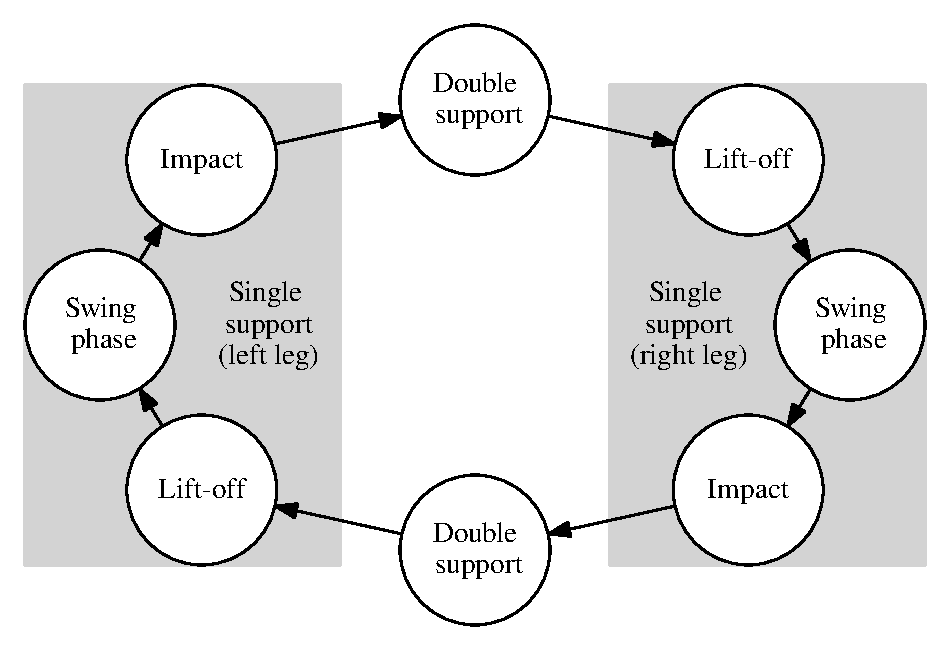
\includegraphics[scale=0.6]{walk_cycle.eps}}
    \caption[Walking cycle of a biped.]{
    Walking cycle of a biped including two \tn{single support} phases, when
    only one foot is on the ground, and two \tn{double support} phases, when
    both feet are on the ground. One single support and one adjacent double
    support comprise a \tn{step}.
    }
    \label{fig.walkcycle}
\end{figure}
%

This goal can be achieved without any actuation by specially designed
mechanical systems called \tn{passive walkers} \cite{McGeer1990ijrs}. They
start walking when positioned on sloped surfaces, where the gravitational force
allows to restore energy lost at foot impacts. Walking on a flat ground can be
enabled by exploiting different sources of energy, for example, heating of the
feet \cite{Nemoto2015iros} or limited actuation \cite{Collins2005science}.
During the walk, the state of passive walkers evolves along a semi-stable limit
cycle $\SET{T}$, whose basin of attraction is the capture basin $\SET{C}$.
Therefore, they can tolerate small perturbations.


The cyclic nature of walking is also exploited in the control of actuated
robots. In particular, the control of a robot as a hybrid system is
significantly simplified due to the sequence of discrete collision events known
in advance. The design and stability analysis of hybrid system controllers is
often further simplified with the help of \tn{virtual constraints} which shape
the walking motion. This approach is referred in the literature as \tn{hybrid
zero dynamics} or \tn{hybrid restriction dynamics} \cite{Westervelt2003tranac,
Chevallereau2003csm, Grizzle2006isccsp, Westervelt2007locomotion}. Typically,
it deals with only planar walking, however, some attempts have been made to
apply it to three dimensional walking as well \cite{Chevallereau2009tro}. Other
researches have also extended this approach to compliant robots
\cite{Sreenath2010ijrr}.


A completely different approach to generation of periodic gaits was inspired by
the neurobiological research. This research indicated a major role of groups of
neurons which generate periodic signals in locomotion of animals. Emulation of
such groups called \tn{central pattern generators} has been successfully
employed in robot locomotion control, even though the balance of the resulting
motion is not usually rigorously proven  \cite{Fukuoka2003ijrr,
Nakanishi2004ras, Ijspeert2008nn}.


The common disadvantage of all these methods is the lack of flexibility: they
are limited to walking and cannot produce acyclic gaits. Sometimes it is also
unclear how to start and terminate the walk or change the walking gait without
falling.



%%%%%%%%%%%%%%%%%%%%%%%%%%%%%%%%%%%%%%%%%%%%%%%%%%%%%%%%%%%%%%%%%%%%%%%%%%%%%%%%
\subsection{General motion and locomotion}\label{sec.balance_general}

Potential practical applications of humanoid robots, such as disaster response
\cite{DRCsite} or airplane assembly \cite{COMANOIDsite}, lie far beyond the
scope of standing or regular walking. Hence, the problem of balance
preservation while performing much more general motions must be addressed. This
is usually achieved as a by-product of motion planning
\cite{LaValle2006planning}, which ensures execution of the motion goals without
falling. We can perceive the motion planning as a procedure of finding a viable
evolution connecting an initial state $\V{x}_s$ and a final state $\V{x}_f \in
\SET{T}$. Whenever $\V{x}_s \notin \SET{C}$ the procedure must necessarily
fail. Note that the sets $\SET{T}$ and $\SET{C}$ are assumed to be defined
based on the constraints taking into account all possible failures.


Determination of a single viable evolution appears to be easier than
determination of the whole $\SET{V}$ and $\SET{C}$ sets. Nevertheless, it is a
very challenging problem, which is usually solved with the help of various
approximations and heuristics. Motion planning in complex situations is often
decoupled into several stages \cite[Chapter~14]{LaValle2006planning}. This
strategy is ubiquitous in planning for legged robots. One of the most commonly
used stages is planning of \tn{stances} -- configurations of the contacts of
the robot with the environment \cite{Bouyarmane2012adrob, Bretl2006ijrr,
Zucker2011ijrr}. Note that, as we have already indicated in
\cref{sec.balance_as_viability}, some of the constraints are neglected on
different stages to reduce computational costs.


An important property of a planning algorithm is \tn{completeness}, \IE, the
ability to find a solution if one exists. In the case of legged robots, it is
common to resort to weaker \tn{probabilistic completeness}
\cite{Kuffner2002auro, Hauser2008ijrr, Dalibard2013ijrr, Shkolnik2011ijrr} or
to \tn{resolution completeness} \cite{Zucker2011ijrr}. The former guarantees
that the probability of finding a solution approaches $1$ as the computation
time increases, the latter is valid for certain resolution of the state space.
Sometimes the completeness is sacrificed by the approaches solely based on
optimization, which may get stuck in a local minimum and, therefore, fail to
find a solution \cite{Dai2014humanoids, Kanoun2010ijrr}.


In spite of an abundance of techniques making motion planning computationally
cheap, it still cannot be performed in real-time. Real-time replanning is,
however, crucial for adaptation to unexpected changes in the environment and
compensation for strong external perturbations \cite{Nishiwaki2009ijrr}. One
way to address this issue is to adjust the precomputed plan if the reality
deviates from it. This may still be intractable in real-time, and a more common
alternative is generation of a short-term plan, which we call motion
\tn{anticipation} or motion \tn{preview}. The performance gain in this case is
achieved due to limited preview horizon, lack of completeness, and, in most
cases, approximated representations of the robot \cite{Kajita2003icra,
Nagasaka2012, Audren2014iros, Nishiwaki2009ijrr}. Low computational cost allows
regeneration of a short-term plan at high frequency, which enables highly
reactive motions. Anticipation can be used to return to the precomputed plan or
can even render it unnecessary for simple motions such as locomotion
\cite{Azevedo2002icra, Wieber2006humanoids, Herdt2010auro, Tassa2014icra,
Sherikov2014humanoids}.


A planned motion is balanced if it complies with all the constraints at all
times and terminates in a final state. The final state, however, usually cannot
be reached, when anticipation over a limited horizon is performed.
Consequently, there is a possibility of reaching a non-viable state. We are not
aware of possibilities to ensure viability without knowledge of the viability
kernel $\SET{V}$. Nevertheless, it is possible to ensure more restrictive
capturability by imposing that the robot must be able to stop or reach certain
walking cycle in the end of preview horizon, \IE, by imposing that the
anticipated motion reaches $\SET{T}$ \cite{Sherikov2014humanoids,
Sherikov2015humanoids, Schouwenaars2006thesis}. Existence of a motion complying
with such constraint implies that the current state $\V{x}_0 \in \SET{C}_H$,
where $H$ is the length of the preview horizon. The requirement to stop does
not undermine the execution of the motion goals provided that two conditions
are met:
%
\begin{enumerate}
    \item the preview horizon is regularly shifted in the future and the
        anticipated motion is recomputed,
    \item the preview horizon is long enough.
\end{enumerate}
%
The first condition implies that the moment, when $\SET{T}$ should be reached,
is continuously postponed. Hence, it is not imposed that the robot stops, but
rather that it maintains the capacity to stop, \IE, capturability. The second
condition is also straightforward: if the robot is required to reach $\SET{T}$
the very next moment, it hardly has enough freedom to execute the motion goals.
This naturally leads to the question about sufficient length of the preview
horizon. Currently, we do not have an answer for the general case: the choice
may well be application dependent. However, the existing research on walking of
both humans and robots strongly suggests that the length of a preview horizon
should cover $2$ or $3$ steps \cite{Zaytsev2015icra, Carver2009chaos,
Kajita2003icra, Koolen2012ijrr, Sparrow2005gaitpost, Vukobratovic1970tranbme}.


The idea of maintaining capturability by imposing that $\SET{T}$ is reached at
the end of a preview horizon is recurrent in the literature. Implementation,
however, is dependent on the particular method chosen for anticipation: the
motion may be a result of solution of a boundary value problem, or an \ac{MPC}
problem with terminal constraints \cite{Mansour2011humanoids, Henze2014iros,
Sherikov2014humanoids, Morisawa2007icra, Takenaka2009iros}. The target set
$\SET{T}$ is usually defined so that the robot's ability to stop
\cite{Mansour2011humanoids, Henze2014iros} is ensured or cyclicity of motions
is enforced \cite{Takenaka2009iros}.




%%%%%%%%%%%%%%%%%%%%%%%%%%%%%%%%%%%%%%%%%%%%%%%%%%%%%%%%%%%%%%%%%%%%%%%%%%%%%%%%
%%%%%%%%%%%%%%%%%%%%%%%%%%%%%%%%%%%%%%%%%%%%%%%%%%%%%%%%%%%%%%%%%%%%%%%%%%%%%%%%
%%%%%%%%%%%%%%%%%%%%%%%%%%%%%%%%%%%%%%%%%%%%%%%%%%%%%%%%%%%%%%%%%%%%%%%%%%%%%%%%
\section{Conclusion}\label{sec.conclusion}

We have defined the balance preservation problem using notions of viability
theory and briefly reviewed existing approaches to this problem based on our
definition. Henceforth, we are going to focus on online control and balancing
of humanoid robots performing general motions. We assume that a global motion
plan is not provided or only partial information, such as planned contact
positions, is given. Therefore, we completely rely on motion anticipation with
limited preview horizon. In the preceding section it is indicated, that
capturability can be enforced in such a situation by imposing appropriate
conditions on the final previewed state. Commonly, these conditions ensure the
capacity of the robot to stop or maintain a cyclic motion. We believe the first
option to be more appropriate, since it allows for generation of both cyclic
and acyclic motions. Hence, in the following chapters we narrow the notion of
capturability by assuming that it implies the capacity of the robot to reach a
statically balanced state, \IE, to stop.
